\documentclass[a4paper]{article}

%use the english line for english reports
%usepackage[english]{babel}
\usepackage[portuguese]{babel}
\usepackage[utf8]{inputenc}
\usepackage{indentfirst}
\usepackage{graphicx}
\usepackage{verbatim}


\begin{document}

\setlength{\textwidth}{16cm}
\setlength{\textheight}{22cm}

\title{\Huge\textbf{Syrtis}\linebreak\linebreak\linebreak
\Large\textbf{Relatório Intercalar}\linebreak\linebreak
\linebreak\linebreak

\includegraphics[scale=0.1]{feup-logo.png}\linebreak\linebreak
\linebreak\linebreak
\Large{Mestrado Integrado em Engenharia Informática e Computação} \linebreak\linebreak
\Large{Programação em Lógica}\linebreak
}

\author{\textbf{Grupo 79:}\\
Flávio Couto - 201303726 \\
Pedro Afonso Castro - 201304205 \\
\linebreak\linebreak \\
 \\ Faculdade de Engenharia da Universidade do Porto \\ Rua Roberto Frias, s\/n, 4200-465 Porto, Portugal \linebreak\linebreak\linebreak
\linebreak\linebreak\vspace{1cm}}

\maketitle
\thispagestyle{empty}

%************************************************************************************************
%************************************************************************************************

\newpage

%Todas as figuras devem ser referidas no texto. %\ref{fig:codigoFigura}
%
%%Exemplo de código para inserção de figuras
%%\begin{figure}[h!]
%%\begin{center}
%%escolher entre uma das seguintes três linhas:
%%\includegraphics[height=20cm,width=15cm]{path relativo da imagem}
%%\includegraphics[scale=0.5]{path relativo da imagem}
%%\includegraphics{path relativo da imagem}
%%\caption{legenda da figura}
%%\label{fig:codigoFigura}
%%\end{center}
%%\end{figure}
%
%
%\textit{Para escrever em itálico}
%\textbf{Para escrever em negrito}
%Para escrever em letra normal
%``Para escrever texto entre aspas''
%
%Para fazer parágrafo, deixar uma linha em branco.
%
%Como fazer bullet points:
%\begin{itemize}
	%\item Item1
	%\item Item2
%\end{itemize}
%
%Como enumerar itens:
%\begin{enumerate}
	%\item Item 1
	%\item Item 2
%\end{enumerate}
%
%\begin{quote}``Isto é uma citação''\end{quote}


%%%%%%%%%%%%%%%%%%%%%%%%%%
\section{O Jogo Syrtis}

\subsection{História}

	O Syris é um jogo de estratégia em que os dois jogadores se encontram numa ilha instável e desconhecida. A paisagem da ilha está sempre em mudança, e o avanço do mar faz com que a ilha esteja a tornar-se cada vez mais pequena... Apenas um dos jogadores poderá sobreviver na ilha, qual conseguirá?
	
\subsection{Objetivo}
	
	A cada jogador é atribuída uma forma e uma cor (quadrado e preto ou círculo e branco). O objetivo do jogo é conquistar todas as peças que contenham a sua cor ou a sua forma.
	
\subsection{Equipamento}

	O jogo é composto por peças quadradas com uma determinada forma e cor. Há 4 combinações possíveis: círculos e quadrados brancos e pretos. Há também quatro torres, duas brancas e circulares e duas pretas e quadradas.
	
\subsection{Preparação}

	As peças quadradas são inicialmente aleatoriamente dispostas num de dois formatos de ilha. Para um jogo mais longo e estratégico, utiliza-se o formato Syrtis Major. Para um jogo mais curto e tático, utiliza-se o formato Syrtis Minor. As figuras \ref{fig:syrtismajor} e \ref{fig:syrtisminor} mostram a estrutura destes dois formatos.
	
\begin{figure}[h]

\begin{minipage}{0.5\linewidth}
\centering
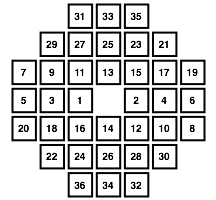
\includegraphics[scale=0.9]{syrtismajor.png}
\caption{Syrtis Major}
\label{fig:syrtismajor}
\end{minipage}
\quad
\begin{minipage}{0.5\linewidth}
\centering
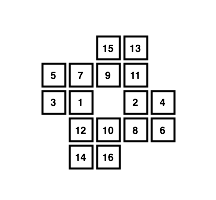
\includegraphics[scale=0.9]{syrtisminor.png}
\caption{Syrtis Minor}
\label{fig:syrtisminor}
\end{minipage}

\end{figure}

Depois, um dos jogadores coloca as 4 torres por cima de uma das peças à sua escolha, desde que sejam da cor ou da forma dessa peça. O outro jogador decide se quer jogar com as torres brancas circulares ou pretas quadradas e o jogo começa por quem tiver ficado com as peças brancas e circulares.

\subsection{Ilhas}

Uma ilha é uma peça ou um grupo de peças que partilham a mesma forma ou cor. Para serem consideradas uma ilha, devem estar adjacentes horizontal ou verticalmente. Há quatro tipos de ilhas: ilhas pretas, brancas, quadradas e circulares. Uma peça pode obviamente pertencer a uma ilha de uma cor e a uma ilha de uma forma ao mesmo tempo. As figuras \ref{fig:circleisland} e \ref{fig:blackisland} mostram exemplos de ilhas.

\begin{figure}[h]

\begin{minipage}{0.5\linewidth}
\centering
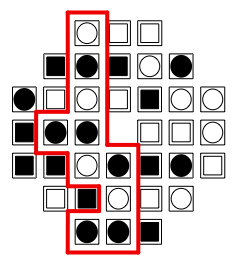
\includegraphics[scale=0.75]{island1.png}
\caption{Ilha de círculos}
\label{fig:circleisland}
\end{minipage}
\quad
\begin{minipage}{0.5\linewidth}
\centering
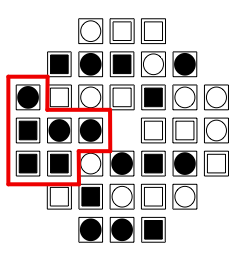
\includegraphics[scale=0.75]{island2.png}
\caption{Ilha de pretos}
\label{fig:blackisland}
\end{minipage}

\end{figure}


\subsection{Acções}

Em cada turno cada jogador pode fazer uma de entre 4 acções possíveis: mover uma torre, afundar uma peça, deslocar uma peça, ou passar a sua vez.

\subsubsection{Mover uma torre}

Cada jogador pode mover uma das suas torres, desde que se mantenha em pelo menos uma das suas duas ilhas atuais (ou seja, ou na ilha respeitante à forma ou na ilha respeitante à cor). As outras torres não bloqueiam este movimento, ou seja, podemos passar por cima de outras torres.  A figura \ref{fig:towermovement} mostra um exemplo do movimento de uma torre.

\begin{figure}[h]
\centering
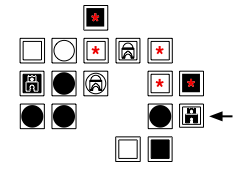
\includegraphics[scale=0.5]{towermovement.png}
\caption{Movimento de uma torre}
\label{fig:towermovement}
\end{figure}

A torre indicada (preta e quadrada) pode mover-se para qualquer uma das peças marcadas com uma seta, pois estas encontram-se na sua ilha quadrangular. Note-se também que ela não pode ir para a peça à sua esquerda, visto que, apesar de ser preta, esta não se encontra na sua ilha (visto que a peça em que a torre se encontra é branca e quadrada, e a peça em questão é preta e circular).

%%%%%%%%%%%%%%%%%%%%%%%%%%
\section{Representação do Estado do Jogo}

Descrever a forma de representação do estado do tabuleiro (tipicamente uma lista de listas), com exemplificação em Prolog de posições iniciais do jogo, posições intermédias e finais, acompanhadas de imagens ilustrativas.


%%%%%%%%%%%%%%%%%%%%%%%%%%
\section{Visualização do Tabuleiro}

Descrever a forma de visualização do tabuleiro em modo de texto e o(s) predicado(s) Prolog construídos para o efeito.
Deve ser incluída pelo menos uma imagem correspondente ao output produzido pelo predicado de visualização.


%%%%%%%%%%%%%%%%%%%%%%%%%%
\section{Movimentos}

Elencar os movimentos (tipos de jogadas) possíveis e definir os cabeçalhos dos predicados que serão utilizados (ainda não precisam de estar implementados).


\end{document}
